%!TEX root = report.tex
\section{Methods \label{chapter2}}
A neural network is a machine learning model that uses a network of functions in multiple layers to understand and translate data inputs into a desired outputs \citep{Bishop:2006:PRM:1162264}.
In classification problems, it learns from extracting the features of many labelled training samples that are usually hidden, and compares its predicted outputs against the given labels.
For each iteration, the loss function is propagated back through the network,
to adjust the weights in each layer.
This process is repeated until a desired accuracy is achieved.
The training algorithm is often referred to as a backward propagation algorithm,
which is useful for training multi-layer feed forward neural networks.

We build a fully connect feed forward neural network for the classification task with a cross-entropy loss and $L2$ weight decay regularisation. Our neural networks implements the Xavier uniform initialisation and three activation layers (Figure~\ref{fig:nn}). 
\begin{figure}
    \centering
    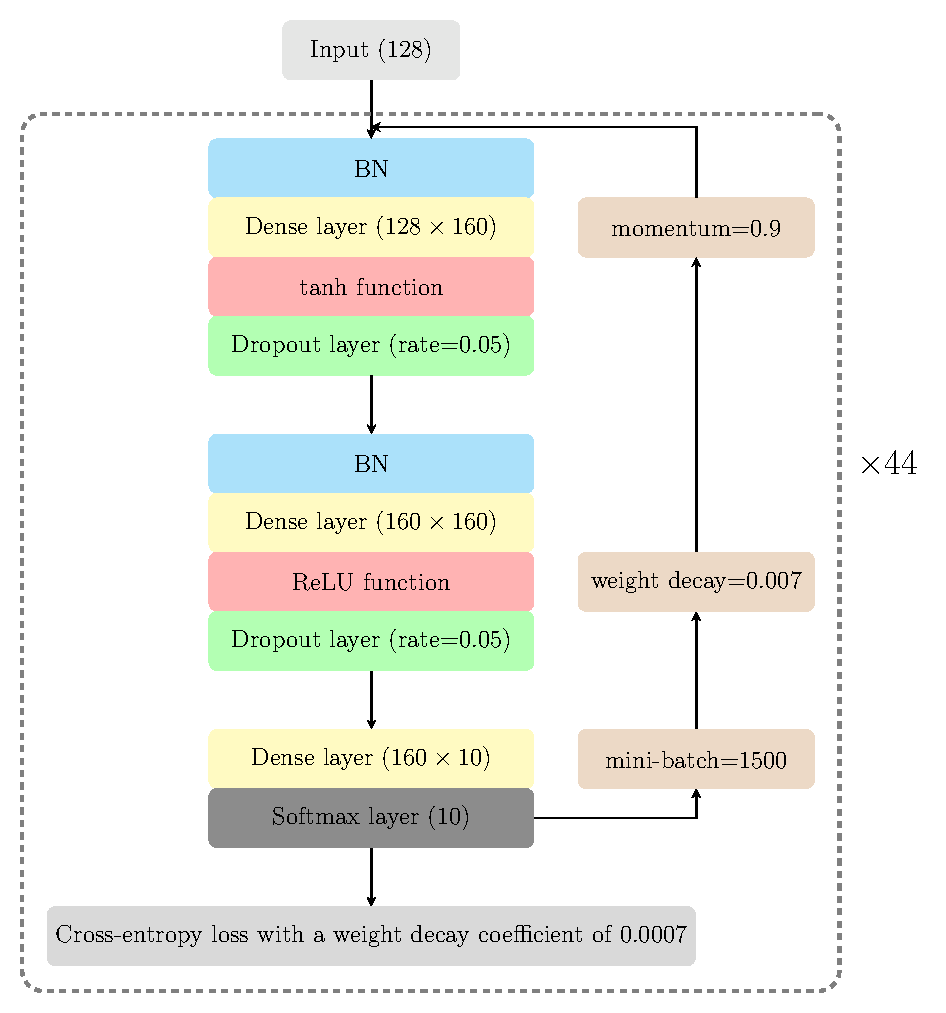
\includegraphics[scale=0.77]{NN.pdf}
    \caption{A diagram illustrates the architecture of our benchmark neural network model. The weights of the densely connected layers are initialised by a uniform distribution proposed by \citet{pmlr-v9-glorot10a}.}
    \label{fig:nn}
\end{figure}
This report uses $\vec t_i=(t_{i1},t_{i2},\ldots)$ to denote the inputs of the $i$th densely connected layer ($i=1,2,3$)
\footnote{We use $(\ )$ to denote column vectors, and $[\ ]$ to denote row vectors.}
, and uses $\vec z_i=(z_{i1},z_{i2},\ldots)$ to denote the outputs of the $i$th activation layer. 
We apply batch normalisation (BN) to normalise the input data~from $\vec t_1$ to~$\tilde{\vec t}_1$. This is followed by a nonlinear activation function. After the first hidden layer, our neural network applies a dropout layer, followed by an additional BN to the normalised outputs. 
We then apply an densely connected layer with a ReLU activation function, an additional dropout layer. The neural network finishes with a Softmax activation layer. 

\subsection{Cross validation score and early stopping prevents overfit\label{sec:early}}
We partition our dataset into $50,000$ training samples and $10,000$ test samples. For each epoch, we first train our model using the training samples and then compute the CV accuracy using the test samples. After $200$ epoch, we find the number of epoch~\texttt{n\_iter} corresponding to the maximum CV accuracy as our early stopping point. Using all the $60,000$ samples, we then train our model again  \texttt{n\_iter} epoches to obtain our final neural network model.

\subsection{Cross-entropy with weight decay improves the model robustness}
Define~$\vec y_k:=(y_{1k},y_{2k},\ldots,y_{10k})$ as the one hot encoding of the training label for the $k$th sample and $\vec p_k:=(p_{1k},p_{2k},\ldots,p_{10k})$ as the corresponding predicted probabilities. We apply the cross-entropy loss to train our neural network
\begin{equation}
  {L(\vec p|\vec y)=-\sum_{k}\sum _{j=1}^{10} y_{jk}\log p_{jk}}.  \label{eq:loss}
\end{equation}

Although the structure of our neural network is relative simple, it still has too many parameters. For example, if we set the number of hidden nodes in each hidden layer to be 160, then the number of parameters to estimate in the weights~$W_1,W_2$ and $W_3$ is $128*160+160*160+160*10=47,680$. The total number of parameters including biases~$b_i$ and BN parameters~$\gamma_i$ and~$\beta_i$ is even greater. As we only have $50,000$ training samples, allowing entries of the weights~$W_i$ to be arbitrary real number overfits the dataset. To encounter this ill-proposed problem, we penalise the complexity of our model by a $L2$ weight decay regularisation term as proposed by \citet{NIPS1991563} and \citet{doi:10.1080/00401706.1970.10488634}
\begin{equation}
  {L=-\sum_k\sum _{j=1}^{10} y_{jk}\log p_{jk}}+\lambda\sum _{i=1}^3\left|W_i\right|^2,  \label{eq:loss_reg}
\end{equation}
where hyperparameter~$\lambda$ is a positive real number.
In comparison with loss function~\eqref{eq:loss}, the regularised loss function~\eqref{eq:loss_reg} penalises the model to have large weight matrices~$W_i$ and hence reduces the model complexity.

The reason to choose cross-entropy loss lies in its derivative. Taking the derivative of loss function~\eqref{eq:loss_reg}
\begin{equation*}
  \frac{\partial L}{\partial z_{3j}}=\sum_k p_{jk}-y_{jk}+\lambda\frac{\partial }{\partial z_{3j}}\sum _{i=1}^3\left|W_i\right|^2.  
\end{equation*}
This derivative function has a key property that many other loss functions like mean square loss do not have---the larger the errors~$\sum_k p_{jk}-y_{jk}$ is, the faster all the neurons will learn.

\subsection{Xavier initialisation speeds up convergence\label{sec:xav}}
We initialise the weight matrix~$W_i$ for $i=1,2,3$ using Monte Carlo method from a uniform distribution bounded by $\pm \sqrt{6/\left[\dim(z_i)+\dim(t_i)\right]}$ as suggest by \citet{pmlr-v9-glorot10a}. We use $0$s as the initial condition for bias vector~$\vec b$. As a result, the weight decay term helps to prevent the neural network from overfitting.

We also have experimented to use the normal distribution initialisation suggested by \citet{pmlr-v9-glorot10a}, but it is outperformed in accuracy and speed. So, this initialisation method is not discussed here.

Xavier initialisation makes sure the initialised weights and biases are not too far away from the optimal weights and biases \citep{pmlr-v9-glorot10a}. This is essential because a poorly initialised optimisation problem usually either ends up with a solution that is far away from global optimum, or even diverges.

\subsection{Batch normalisation prevents internal covariance shift and smooths optimisation}
We normalise the inputs~$t_{ij}$ for layers~$i=1,2$. When training using mini-batch~$B$ as defined in Section~\ref{sec:minibatch}, we use $\mu_B^{(j)}$ and $\sigma_B^{(j)^2}$ to denote the sample mean and sample variance for the mini-batch~$B$. Here, each of the index~$j$ denotes one dimension of the input data. Moreover, we define $\gamma_{ij}$ and $\beta_{ij}$ ($i=1,2$) as real parameters to be learnt by backward propagation. The BN layer iteratively normalise each dimensions~$j$ of the input batch as
\begin{equation}
     {\tilde {t}}_{ij}=\gamma_{ij}\frac {{t}_{ij}-\mu _{B}^{(j)}}{\sqrt {\sigma _{B}^{(j)^{2}}+10^{-8} }}+\beta_{ij} \text{ where } i=1,2.
\end{equation}
When predicting test labels, we use the training means~$\frac{1}{\left|B\right|}\sum_B \mu_B^{(j)}$ and training  variances~$\frac{1}{\left|B\right|}\sum_B \frac{\left|B\right|}{\left|B\right|-1}\sigma_B^{(j)^2}$ to normalise the test inputs.
Our neural network applies this BN layer to prevents internal covariance shift \citep{pmlr-v37-ioffe15}. In addition, \citet{NIPS20187515} find that BN makes the optimisation landscape considerably smoother.

\subsection{Dropout performs model averaging}
We apply dropout to the inputs of the 2nd and 3rd densely connected layers~$\vec t_2$ and $\vec t_3$, as proposed by \citet{dropout}. 
When training our neural network, the dropout layer randomly ignores neurons in vectors~$\vec t_2$ and $\vec t_3$ with a given probability hyperparameter~$p$. 
When predicting labels for CV samples and testing samples, we multiply weights~$W_i$ where layer index~$i=2,3$ by hyperparameter~$p$. This dropout layer is equivalent to model averaging, and forces our neural network to learn a more robust set of parameters that are useful in conjunction with many distinct random subsets of the neurons \citep{DBLP:journals/corr/abs-1207-0580}.

\subsection{Activation functions map input to desired output range}
Our neural network model has three densely connected layers. These three layers respectively implements a nonlinear activation function ($\tanh$ or sigmoid), a ReLU activation function, and a Softmax activation function.
\subsubsection{Nonlinear activation\label{sec:nonl}}
The first densely connected layer is chosen to be either of a hyperbolic function 
\begin{equation}
 \vec z_1(\tilde{\vec  t}_1)=\tanh(W_1\tilde{\vec  t}_1+\vec b_1) \label{eq:tanh}
\end{equation}
or a sigmoid function 
\begin{equation}
  \vec z_1 (\tilde{\vec  t})_1 =  {\vec 1}\left/\left[\vec 1 + \exp\left(W_1\tilde{\vec  t}_1+\vec b_1 \right)\right]\right.  \label{eq:sig}
\end{equation}
where matrix~$W_1$ is a $160\times128$ weighting matrix and vector~$\vec b$ is an $160$-dimensional bias vector. 
Here, the division~$/$ is an elementwise operator.
This layer provides non-linearity to our neural network.
\subsubsection{ReLU activation function}
The second densely connected layer is the piece-wise linear function named as ReLU
\begin{equation*}
   \vec z_2(\tilde{\vec  t}_2)=\max(0,W_2\tilde{\vec  t}_2+\vec b_2).
\end{equation*} 
ReLU forces the output of the layer to be sparse. In contrast, the nonlinear activation functions~\eqref{eq:tanh} and~\eqref{eq:sig} do not have this property. 
The sparseness makes the neural network more computationally efficient \citep{NIPS20145267}.
\subsubsection{Softmax activation function}
The Softmax activation functions takes a vector of real numbers as the input, and convert it into a categorical distribution as the output. Define matrix~$\mathbf 1$ to be a $10\times 10$ matrix of ones so that pre-multiplying by matrix~$\mathbf 1$ is equivalent to summing up all rows. The activation function is the probability mass function of the categorical distribution
\begin{equation}
     \vec z_{3}(\vec t_3)={\exp(W_3 \vec t_{3}+\vec b)}\left/\left[{\mathbf 1\exp{(W_3 \vec t_{3}+\vec b)}}\right]\right.,
\end{equation}
which sums up to one. We assign the index of probability vector~$\vec z_{3}(\vec t_3)$ corresponding to the largest probability as the classification result for the corresponding sample.

\subsection{Stochastic gradient descent finds the optimal weights}
We use gradient descent with mini-batch and momentum to iteratively find optimise our model.
\subsubsection{Mini-batch improves the speed of computation \label{sec:minibatch}}
Traditional batch gradient descent uses all samples to estimate the gradient of the loss function. Estimating such a gradient using this way may be a very computationally expensive procedure. Alternatively, stochastic gradient descent uses only one sample to estimate the gradient. Although it economises the computational cost, the non-smooth nature makes the convergent much slower. 
We applied mini-batch as a compromise between the true gradient descent and the stochastic gradient descent methods. 
Instead of using either all samples or only using one sample to estimate the gradient, we use $1,500$ training samples (i.e. a ``mini-batch''~$B$) at each step. 
In comparison with stochastic gradient descent, mini-batch naturally takes advantage of the vectorisation nature of the \texttt{numpy} library and converges much faster \citep{DBLP:journals/corr/GoyalDGNWKTJH17}.

\subsubsection{Momentum accelerates rate of convergence}
We use~$\eta$ to denote the learning rate, $\alpha$ to denote the momentum coefficient, $\Delta W_i^{(s)}$ to denote the update of weight~$W_i$ in the $s$th iteration, and $\nabla$ to denote the gradient operator. In the $s$th iteration, recall that the first order Taylor expansion of the loss function~\eqref{eq:loss_reg} informs to update the weight matrix~$W_i$ as $W_i^{(s+1)}:=W_i^{(s)}-\eta\nabla L(W_i^{(s)})$, the gradient descent update with momentum proposed by \citet{rumelhart1986learning} is
\begin{equation*}
    \Delta W_i^{(s+1)}=\alpha \Delta W_i^{(s)}-\eta \nabla L(W_i^{(s)})\text{ and } W_i^{(s+1)}=W_i^{(s)}+\Delta W_i^{(s+1)}.
\end{equation*}
To initialise this update, we set $\Delta W_i^{(0)}:=0$. This autoregressive update proposal smooths the wiggliness caused by gradient descent \citep{rumelhart1986learning}, and hence significantly accelerates the rate of convergence.

%\subsubsection{todo: adam}